\documentclass{article} % For LaTeX2e
\usepackage{nips13submit_e,times}
\usepackage{hyperref}
\usepackage{url}
\usepackage{tikz}
\usepackage{wrapfig}
\usepackage{graphicx}
\usepackage{subfig}

\bibliographystyle{plain}
%\documentstyle[nips13submit_09,times,art10]{article} % For LaTeX 2.09

\title{Learning Human Activities and Object Functionalities through Conditional Random Fields}

\author{
Nakul Gopalan\\
Department of Computer Science\\
Brown University\\
Providence, RI 02912 \\
\texttt{ngopalan@cs.brown.edu} \\
\And
Jun Ki~Lee\\
Department of Computer Science\\
Brown University\\
Providence, RI 02912 \\
\texttt{jklee@cs.brown.edu} \\
}

% The \author macro works with any number of authors. There are two commands
% used to separate the names and addresses of multiple authors: \And and \AND.
%
% Using \And between authors leaves it to \LaTeX{} to determine where to break
% the lines. Using \AND forces a linebreak at that point. So, if \LaTeX{}
% puts 3 of 4 authors names on the first line, and the last on the second
% line, try using \AND instead of \And before the third author name.

\newcommand{\fix}{\marginpar{FIX}}
\newcommand{\new}{\marginpar{NEW}}

\nipsfinalcopy % Uncomment for camera-ready version

\begin{document}

\maketitle

\begin{abstract}
Recognizing a human activity is a skill that humans learn early in life. Activity recognition helps humans in predicting next steps of the activity in question and also in planning other activities with respect to the recognized activity. Our goal is to recognize human activities using machine learning, to predict next steps of an action, or provide help using robots or other interfaces. Specifically, what interests us is the human activities being performed near a table-top table or a shelf, where the human can be observed and helped by a robot. We will use a dataset from \cite{koppula2013detectingactivitiesrgbd} to learn a Graphical Model with temporal and spatial structure, which can then be used to predict the action being performed and functionalities of objects. Both will then be used to recognize a higher level activity. As a baseline we have results of a bag of words classification of the $10$ activities, which yields a result of $67\%$. We will tackle the problem using Conditional Random Fields and try to achieve better performance.
\end{abstract}

\section{Introduction}
Recognizing a human activity is a skill that humans learn early in life. Activity recognition helps humans in predicting next steps of the activity in question and also in planning other activities with respect to the recognized activity. Our objective is to recognize human activities using machine learning, to predict next steps of an action. Recognized actions can provide help to humans using robots or other interfaces. Specifically of interest to us are the human activities being performed on a table-top, where the human can be observed and helped by a robot.

We plan to use a dataset\footnote{\url{http://pr.cs.cornell.edu/humanactitivities}} used in \cite{koppula2013detectingactivitiesrgbd}
 to learn a Graphical Model with temporal and spatial structure, which can then be used to predict the action being performed and functionalities of objects. Both will then be used to recognize higher level activities. This dataset is created from streams of the RGB-D images acquired from a Infrared depth sensing camera. The dataset contains both the tracked human skeletal poses and object locations and supervised labels of sub- and high-level- activities and object functionalities. 
 
Among many works in human activity recognition using RGB-D images, Sung et al. in \cite{sung2012unstructured}
proposed a hierarchical maximum entropy Markov model to detect high level activities and sub-activities. This work only uses human skeletal data. Gall et al. in \cite{gall2011functional} used both the human skeletal data and object tracking data to inference sub-activities and object functionalities. His approach sequentially inferences sub-activities and then object functionalities. It does not take both into account at the same time. Koppula et al. in \cite{koppula2013detectingactivitiesrgbd} and \cite{koppula2013anticipating}, uses both the human skeletal poses and object locations and their relationships to low and high level activities and functionalities of objects using Conditional Random Fields (CRF).

\section{Dataset}
We explored data sets with activity labels and corresponding skeletal trajectories. Humans frequently perform activities using objects, especially in table-top scenarios. The dataset from \cite{koppula2013detectingactivitiesrgbd} was constructed keeping this relationship in mind. The raw data consists of the RGB-D frames from the scenes of humans performing activities and human skeletal poses from the OpenNI NITE tracker \cite{PrimeSense2010}. The skeletal poses are not precise and have confidence intervals. The labels on the data are related to both the objects present in the scene and the activities involved. Activity specific labels are framewise labels on subactivities	and the main activity being performed. The sub-activity labels are that of \textit{reaching, moving, pouring, eating, drinking, opening, placing, closing, scrubbing} and \textit{null}. The object specific data consist of object locations for each time frame per object with its object id and its affordance present in the scene. The object affordance labels are those of \textit{reachable, movable, pourable, pour to, containable, drinkable, openable, placeable, closable, scrubbable, scrubber} and \textit{stationary}. The dataset also has precomputed features that have relationship between objects and skeletal poses across frames. 
For the experiments performed in this proposal we use only skeleton pose data, but for our next set of results we would use the pairwise relationship between objects and the skeleton data, and also the temporal features of data available.

\section{Methods}
The data from \cite{koppula2013detectingactivitiesrgbd} has both temporal and spatial structure. For example, the spatial structure has relationships between objects and skeleton positions within a frame. There is also a temporal relationship between previous skeletal pose and object positions and those of the current frame. The authors from \cite{koppula2013detectingactivitiesrgbd} modelled this structure using a pairwise Conditional Random Field(\cite{sutton06introduction}) as shown in 
Fig.~\ref{fig:model}. 
Here each node corresponds to an object or a subactivity. The object nodes can take any of the $12$ possible affordace labels and the subactivity nodes can take any of the $10$ possible labels. The affordance and subactivity nodes are hidden, but feature values for label assignments over the nodes can be computed. The authors in \cite{koppula2013detectingactivitiesrgbd} first predicted sub-activity labels and object affordances, i.e. inference over the model, and then used an SVM to predict the label of the over all activity. To predict the sub-activity and object affordance labels the authors used a maximum energy formulation, where the labels that lead to the maximum possible energy together are accepted. This energy is a sum of products of features and feature weights. Hence we need to learn the weights of the features first, which is performed in the learning stage, with the supervised labelled input from the dataset discussed above, such that training error is minimum. We plan to run the complete experiments ourselves with different features that the ones the authors used, or create some some more. Then perform the learning and inference, and compare our results to those from the original paper. 

As a baseline for our experiments we classify high level activities from skeletal trajectories using a Bag of Words model \cite{Sivic03} with skeletal poses as features. We have about $8$ examples per activity for training and $4$ examples per activity for testing. Each frame has a skeletal pose, of $170$ dimensions, and each activity has about $400$ frames. We cluster skeletal poses over all activities into $200$ clusters using k-means. Now for each activity label we create a histogram by counting clusters closest to each of the poses, and each activity has a histogram word. Now for each test activity we find the nearest neighbour word from the trained histogram words and return its label. The accuracy of this simple Bag of Words model is about $67.3\%$.  In the next section we have attached a schedule that we will follow over the course of the project.

\begin{figure}[t]
\centering
\subfloat[]
{
\label{fig:model}
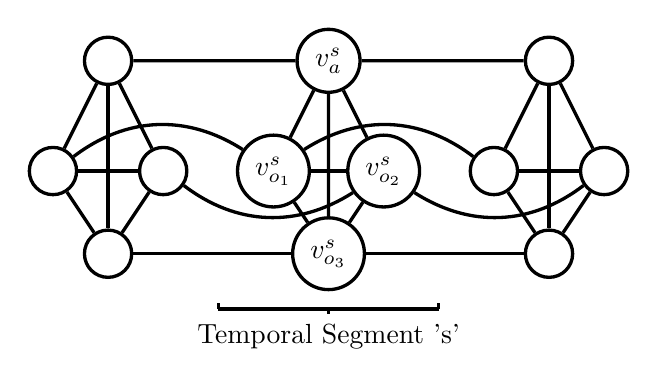
\begin{tikzpicture}[scale=0.7, -,auto,very thick,main node/.style={circle,draw, minimum size=0.6cm}]
  \node[main node] (a1) at (1, 3.5) {};
  \node[main node] (a2) at (1, 0) {};
  \node[main node] (a3) at (0, 1.5) {};
  \node[main node] (a4) at (2, 1.5) {};
  \node[main node] (b1) at (5, 3.5) {$v_a^s$};
  \node[main node] (b2) at (5, 0) {$v_{o_3}^s$};
  \node[main node] (b3) at (4, 1.5) {$v_{o_1}^s$};
  \node[main node] (b4) at (6, 1.5) {$v_{o_2}^s$};
  \node[main node] (c1) at (9, 3.5) {};
  \node[main node] (c2) at (9, 0) {};
  \node[main node] (c3) at (8, 1.5) {};
  \node[main node] (c4) at (10, 1.5) {};
  \path
	(a1) edge (a2)
    (a1) edge (a3)
    (a1) edge (a4)
    (a2) edge (a3)
    (a2) edge (a4)
    (a3) edge (a4)
	(b1) edge (b2)
    (b1) edge (b3)
    (b1) edge (b4)
    (b2) edge (b3)
    (b2) edge (b4)
    (b3) edge (b4)
	(c1) edge (c2)
    (c1) edge (c3)
    (c1) edge (c4)
    (c2) edge (c3)
    (c2) edge (c4)
    (c3) edge (c4)
    (a1) edge (b1)
    (b1) edge (c1)
    (a2) edge (b2)
    (b2) edge (c2)
    (a3) edge [bend left=35] (b3)
    (b3) edge [bend left=35] (c3)
    (a4) edge [bend right=35] (b4)
    (b4) edge [bend right=35] (c4);
  \draw[very thick] (3, -1)--(7, -1);
  \draw[very thick] (3, -1)--(3, -0.9);
  \draw[very thick] (7, -1)--(7, -0.9);
  \draw[very thick] (5, -1)--(5, -1.1);
  \node at (5, -1.5) {Temporal Segment 's'};
\end{tikzpicture}
}
\hspace{1mm}
\subfloat[]
{
\label{fig:image}
\includegraphics[height=4cm]{images/RGB_137.png}
}
\caption{ \textbf{(a)} an example of a Conditional Random Field used in \cite{koppula2013detectingactivitiesrgbd}. Each temporal segment (s) has one sub-activity node $v_a^s$ and three object nodes $\{ v^s_{o_1}, v^s_{o_2}, v^s_{o_3} \}$, \textbf{(b)} an example image from the data set}
\end{figure}

\section{Schedule}
\begin{description}
\item[Week 0] ($\sim$11/11/14) Understanding the data set and running bag-of-worlds model classifier on the raw data set to classify high-level actions.
\item[Week 1] ($\sim$11/18/14) Extracting features from the raw data set.
\item[Week 2] ($\sim$11/25/14) Modelling Conditional Random Fields (CRFs) 
\item[Week 3] ($\sim$12/02/14) Implementing the CRFs and Implementing Optimization Techniques
\item[Week 4] ($\sim$12/09/14) Pulling out the final result and Presentation Preparation
\item[Week 5] ($\sim$12/16/14) Pulling out the final result and write ups.
\end{description}

\bibliography{ref}

\end{document}
